\section{On interpretation of power spectra of POD mode chronos}
\label{app:fourier}
\paragraph{Fourier transform of POD mode chronoses}
Let us assume a continuous counterpart of the decomposition~\eqref{eq:chronosTopos},
\begin{equation}
\label{eq:continuousDiadPairs}
    y(\bm{x},t) = \sum\limits_{(j)}\psi_{j}(\bm{x})\otimes \eta_{j}(t)\,,\quad \bm{x}\in\Omega\,,\quad t\in (0,T]\,,
\end{equation}
where $y$ is a general function $y:\Omega\times (0,T] \rightarrow \mathbb{R}$, and $\Omega\subset \mathbb{R}^{3}$ is a bounded connected domain. Furthermore, $(\psi_{j},\eta_{j})$ is the dyadic pair forming the $j$-th mode, where $\psi_{j}$ and $\eta_{j}$ are the $j$-th topos and chronos, respectively.

The standard approach to study the dynamics of $y$ via spectra obtained by the Fourier transform is to select a number of probe points $\bm{p}_{i}\in\Omega\,,\,i=1,\dots,n_{p}$, focus on $y_{p_{i}}(t):=y(\bm{p}_{i},t)$, compute the Fourier transforms $\hat{y}_{p_{i}}(f)\xleftarrow{\mathcal{F}} y_{p_{i}}(t)$, and to analyse the resulting spectra $\hat{y}_{p_{i}}(f)\,,\,i=1,\dots,n_{p}$ where $f$ is the frequency in the Fourier space. A similar approach was applied to obtain the results given in Figure~\ref{fig:turbSpectraPts}.

Focusing on the decomposition~\eqref{eq:continuousDiadPairs}, note that the information on the dynamics of $y$ is contained only in the chronoses $\eta_{j}$. For the sake of argument, let us now assume that $y(\bm{x},t) \equiv y(\bm{p}_{i},t) =: y(t)$ and $\psi_{j}$ in~\eqref{eq:continuousDiadPairs} is merely a real-valued multiplicative constant. Recalling the Fourier tranform linearity, i.e.,
\begin{equation}
\label{eq:fourierLin}
    \begin{array}{c}
        \displaystyle y(t) = \sum\limits_{(j)}c_{j}\eta_{j}(t) \iff \hat{y}(f) = \sum\limits_{(j)}c_{j}\hat{\eta}_{j}(f),\,\quad\forall c_{j}\in\mathbb{C}\,,\\[0.4cm]
        y(t) \xrightarrow{\mathcal{F}} \hat{y}(f)\,,\quad\eta_{j}(t) \xrightarrow{\mathcal{F}} \hat{\eta}_{j}(f)\,,
    \end{array}
\end{equation}
the spectrum of $y(t)$ is a sum of the spectra of individual modes chronoses $\eta_{j}(t)$.

Now, moving from $\Omega$ to its discretization $\Omega^{h}$ with $m$ discretization points, the relation~\eqref{eq:continuousDiadPairs} is transformed as
\begin{equation}
\label{eq:semiDiscDiadPairs}
    \bm{y}(t) = \sum\limits_{j=1}^{m}\bm{\psi}_{j} \eta_{j}(t)\,,\quad \bm{\psi}_{j}\in\mathbb{R}^{m}\,,\,\bm{\psi}_{i}\cdot\bm{\psi}_{j}=\delta_{ij}\,,\, t\in (0,T]\,,
\end{equation}
where $\delta_{ij}$ is the Kronecker delta and $\bm{y}:(0,T]\rightarrow \mathbb{R}^{m}$ is a trajectory of an unspecified dynamical system. Treating~\eqref{eq:semiDiscDiadPairs} component-wise, i.e. as indicated in~\eqref{eq:fourierLin}, one arrives at
\begin{equation}
\label{eq:}
    \hat{\bm{y}}(f) = \sum_{j=1}^{m}\bm{\psi}_{j}\hat{\eta}_{j}(t)\,,
\end{equation}
i.e. the spectrum of the original variable may be reconstructed from the spectra of chronoses. Furthermore, the POD modes $(\bm{\psi}_{j},\eta_{j})$ are ordered in a way that each partial sum $\bm{y}^{\ell}(t) = \sum_{j=1}^{\ell < m}\bm{\psi}_{j} \eta_{j}(t)$ is the optimal approximation of $\bm{y}$ by $\bm{y}^{\ell}$ with respect to the error in the Frobenius norm ($\norm{\bm{y}-\bm{y}^{\ell}}_{F}$). The relative contribution of each mode to the minimization of the approximation error is proportional to the amplitude of $\eta_{j}$, i.e. to the singular value $\sigma_{j}$, see~\eqref{eq:svdY}.

\paragraph{Analysis of laminar von Karman vortex street}
To illustrate the applicability of the above outlined Fourier transform properties to an analysis of a system dynamics via power spectra of POD chronoses, let us concentrate on a simplified case of a laminar von Karman vortex street. In particular, the examined case corresponds to a two-dimensional approximation of a vortex shedding behind a circular cylinder at $\Rey = 115$.

\begin{figure}[htbp]
    \centering
    % \begin{tikzpicture}
	\begin{axis}[
		name=plot1,
		xlabel={$f\,\mathrm{[Hz]}$},
		ylabel={$E_i\,\mathrm{[a.u.]}$},
		font = \scriptsize,
		width=0.98\textwidth,
		height=0.6\textwidth,
		ytick pos=left,
		xtick pos=bottom,
		ymode=log,
		xmode=log,
		line width = 0.85pt,
		xmax=7,
		xmin=0.25,
        ymin=1e-9,
        ymax=1e3,
        xtick={0.5,1,2,4,6},
        log x ticks with fixed point,
        legend style ={
                at={(0.01,0.99)}, 
                anchor=north west,
                draw=black, 
                fill=white,
                align=right,
                legend columns=3,
                font=\scriptsize
            },
		]
        \draw[line width = 0.55pt] (axis cs:1.42391,1e-9) -- (axis cs:1.42391,1e3) node [left,anchor=east] at (axis cs:1.42391,0.5e-8) {$f_{1}^{\mathrm{lam.}}$};
        \draw[line width = 0.55pt,dashed] (axis cs:2.84782,1e-9) -- (axis cs:2.84782,1e3) node [left,anchor=east] at (axis cs:2.95,3e2) {$f_{2}^{\mathrm{lam.}}$};
        \draw[line width = 0.55pt,dashdotted] (axis cs:4.27173,1e-9) -- (axis cs:4.27173,1e3) node [left,anchor=east] at (axis cs:4.4,3e2) {$f_{3}^{\mathrm{lam.}}$};
        \draw[line width = 0.55pt,dotted] (axis cs:5.71542,1e-9) -- (axis cs:5.71542,1e3) node [left,anchor=east] at (axis cs:5.9,3e2) {$f_{4}^{\mathrm{lam.}}$};
        
		\addplot [color=blue,mark=none,select coords between index={1}{400},smooth] table [x expr=\thisrow{f}, y expr = 1e3*\thisrow{eta0}^2]{\myGraphs/lamVKStreet/scaledEtas0-7Re115PP.dat};\label{eta0}
        \addlegendentry{$\hat{\eta}_{1}$};
		\addplot [color=red,mark=none,select coords between index={1}{400},smooth] table [x expr=\thisrow{f}, y expr = 1e3*\thisrow{eta2}^2]{\myGraphs/lamVKStreet/scaledEtas0-7Re115PP.dat};\label{eta2}
        \addlegendentry{$\hat{\eta}_{3}$};
        \addplot [color=green!70!black,mark=none,select coords between index={1}{400},smooth] table [x expr=\thisrow{f}, y expr = 1e3*\thisrow{eta4}^2]{\myGraphs/lamVKStreet/scaledEtas0-7Re115PP.dat};\label{eta4}
        \addlegendentry{$\hat{\eta}_{5}$};
        \addplot [color=brown,mark=none,select coords between index={1}{400},smooth] table [x expr=\thisrow{f}, y expr = 1e3*\thisrow{eta6}^2]{\myGraphs/lamVKStreet/scaledEtas0-7Re115PP.dat};\label{eta6}
        \addlegendentry{$\hat{\eta}_{7}$};
        \addplot [color=black,mark=none,select coords between index={1}{400},smooth] table [x expr=\thisrow{f}, y expr = 1e3*\thisrow{sumEtaSq}]{\myGraphs/lamVKStreet/scaledEtas0-7Re115PP.dat};\label{etaS}
        \addlegendentry{$\sum_{j=1}^{8}\hat{\eta}_{j}$};
        \addplot [color=gray,mark=none,select coords between index={1}{600},smooth] table [x expr=\thisrow{f}, y expr = \thisrow{spct}^2/5]{\myGraphs/lamVKStreet/probe1_V.dat};\label{vPt}
        \addlegendentry{$\hat{v}$};
	\end{axis}
\end{tikzpicture}

    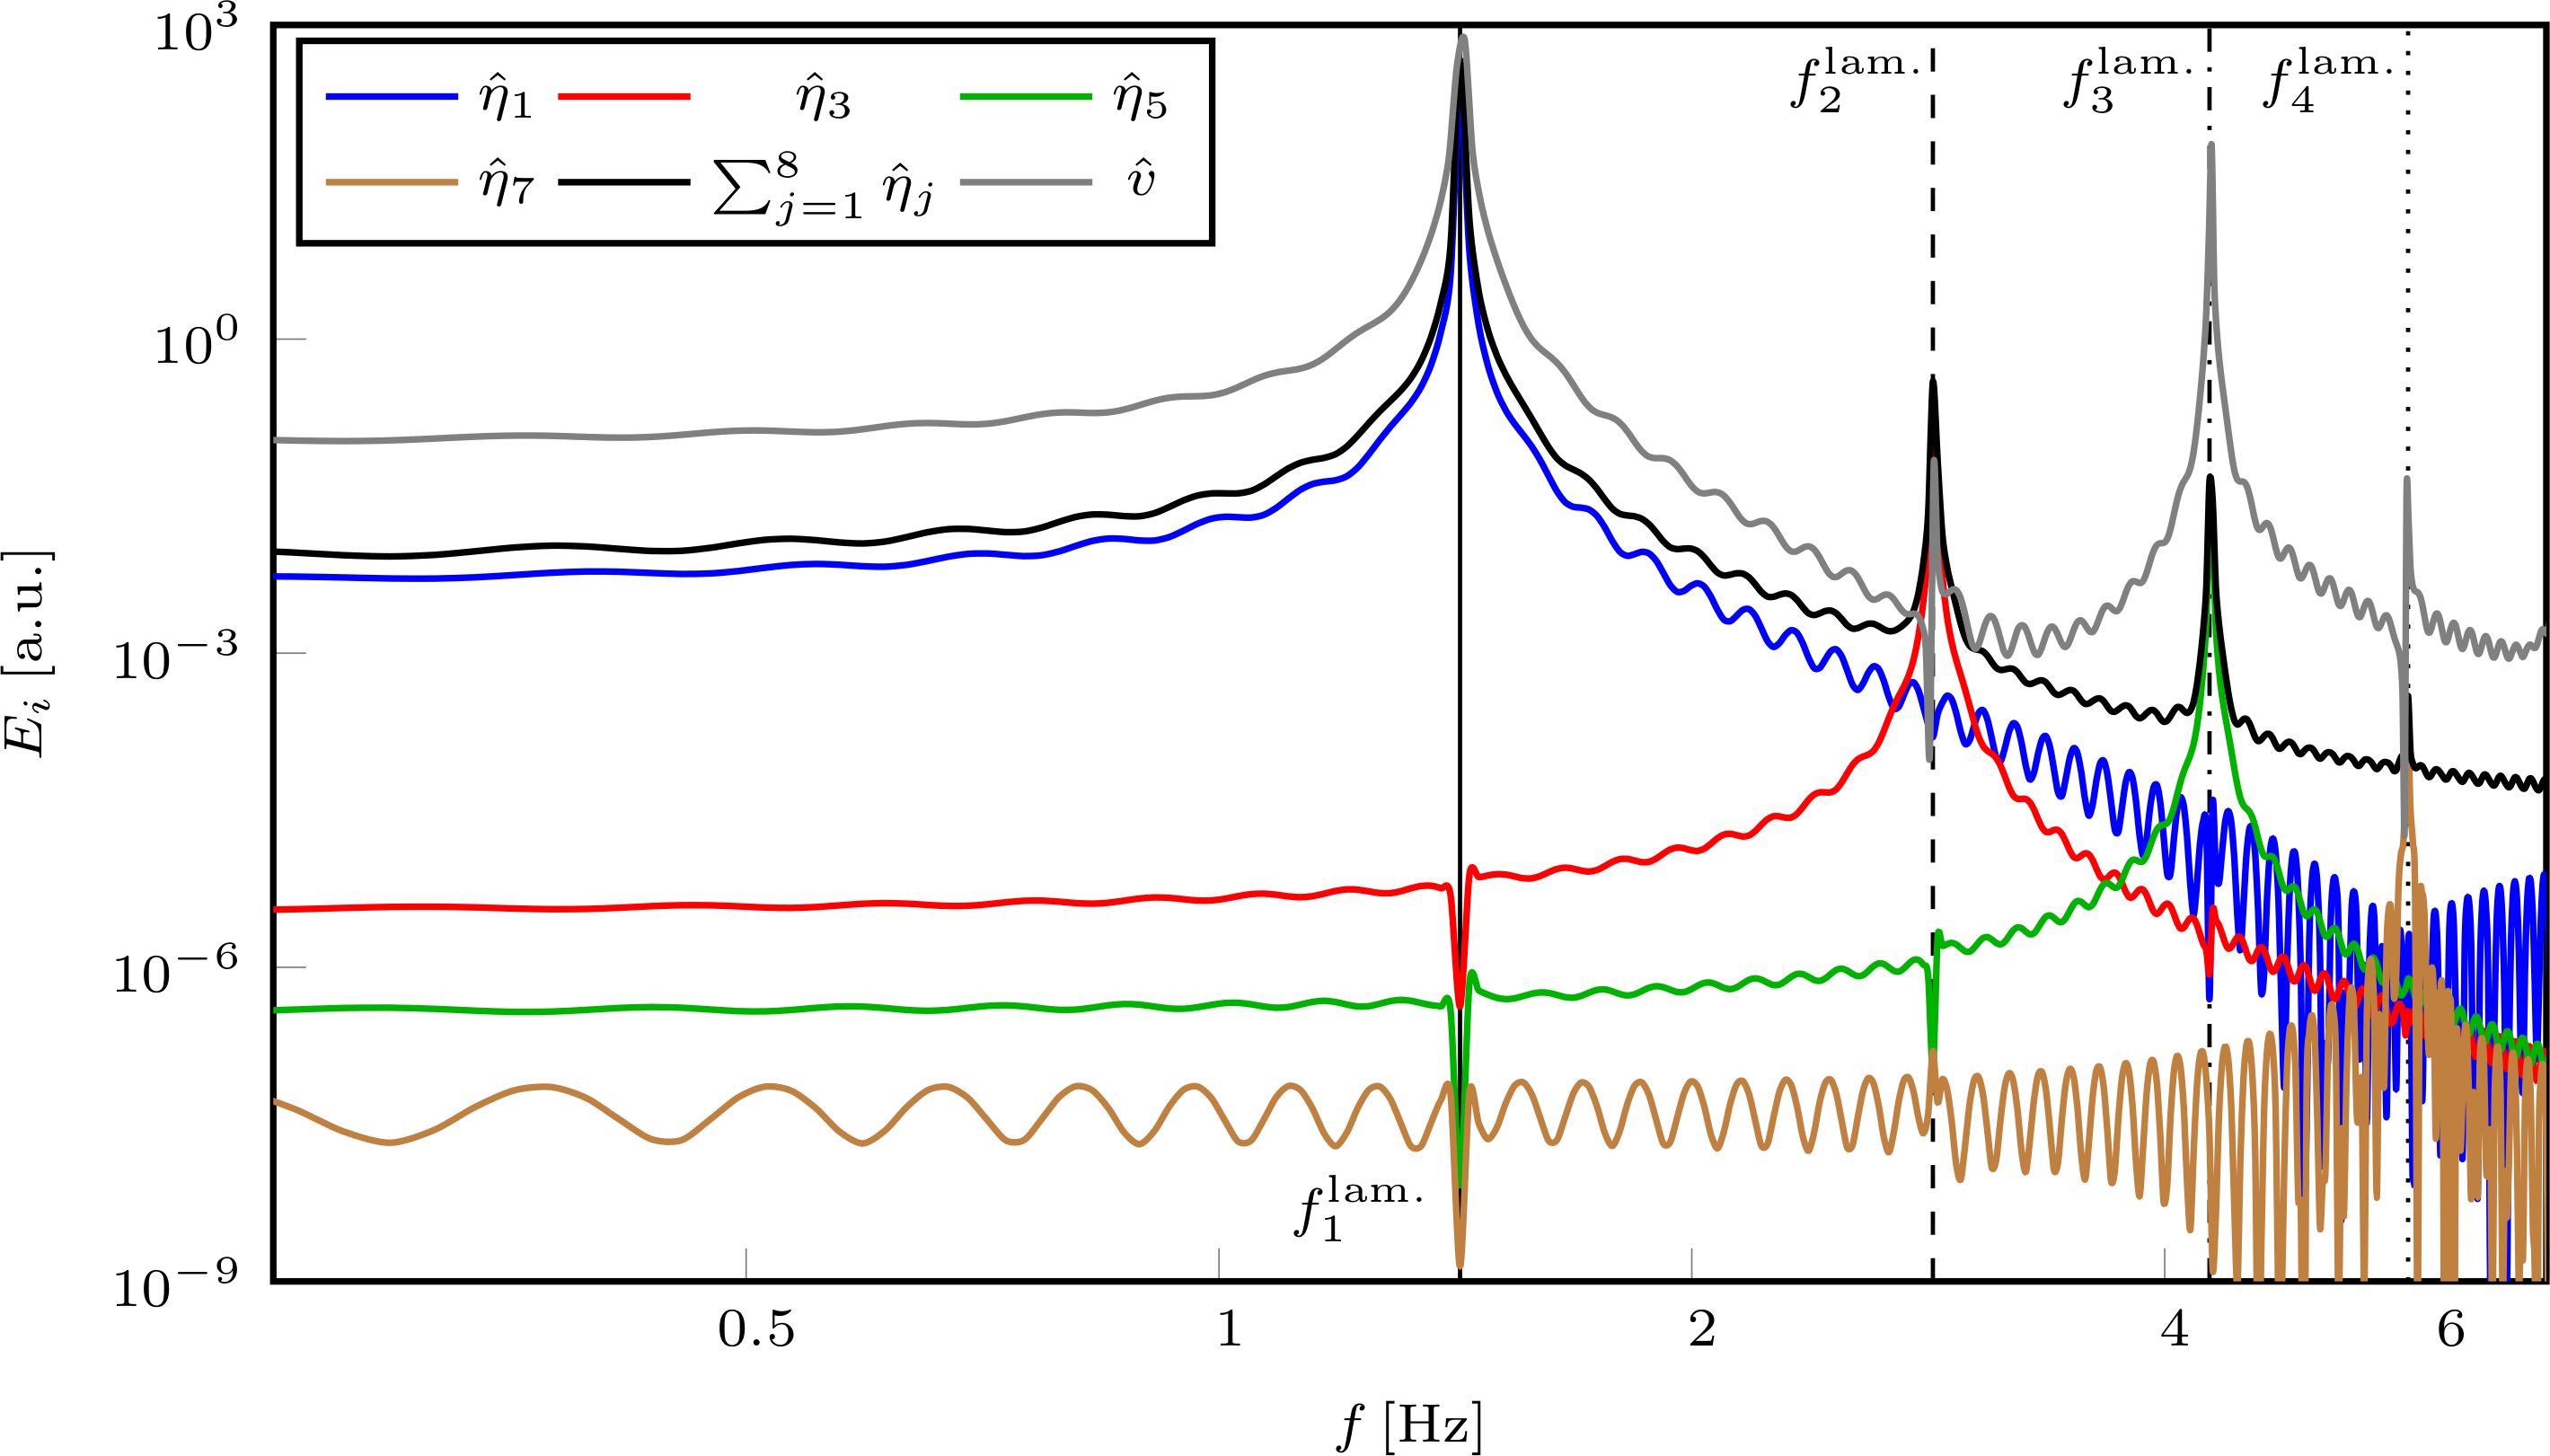
\includegraphics[width=0.98\textwidth]{02_images/00_export/figure26.png}
    \caption{Dynamics of vortex shedding behind a circular cylinder at $\Rey = 115$. Spectra $\hat{\eta}_{j}$ obtained by the Fourier transform of $\eta_{i},\,i=1,3,5,6$, scaled by $\sigma_{i}^{2}$ and their sum, compared to the spectrum of $v$ velocity component in the point $p_{1}$ (see Figure~\ref{fig:meansPom1}). Spectra of $\eta_{j},\,j=2,4,6,8$, look qualitatively the same as spectra of their odd counterparts and were omitted for the sake of image clarity.}
    \label{fig:lamVKStreetSpectra}
\end{figure}

The toposes obtained by POD of the studied laminar flow velocity field have a well known structure in which they are organized in pairs representing roughly equivalent portion of the system kinetic energy, i.e. $\sigma_{k}^{2}\approx \sigma_{k+1}^{2},\,k = 2i-1,\,i\in\mathbb{N}$, see, e.g., the work of \citet{taira2020}. As for the flow dynamics, the original flow is periodic. By the argument listed in the previous paragraph, also the mode chronoses exhibit an (almost) periodic behavior. The period of the first mode couple, i.e. modes one and two, corresponds to the principal flow harmonics, the period of the second mode couple to the flow secondary harmonics and so on, see \citep{isoz2018}. Spectra of the first eight modes chronoses for the laminar vortex shedding are, together with their sum and a reference spectrum obtained by an analysis of the $v$ velocity component in the point $p_{1}$, given in Figure~\ref{fig:lamVKStreetSpectra}. The spectrum $\hat{\eta}_{j}$ represent information on the dynamics of the whole spatial structure $\bm{\psi}_{j}$, i.e. an information somehow averaged over the spatial computational domain $\Omega$ and all the velocity components. On the other hand, the spectrum of the original velocity field component $v$ recorded in a single spatial point provides direct, albeit local, information on the original system dynamics.

Note that contrary to the dynamic mode decomposition and related methods, POD is not capable of separating flow structures oscillating at a single frequency, see the higher modes in Figure~\ref{fig:lamVKStreetSpectra}. Still, based on an examination of the mode spectrum $\hat{\eta}_{j}$, it is possible to devise the mode $(\bm{\psi}_{j},\eta_{j})$ qualitative dynamic behavior. Concentrating on the turbulent vortex shedding studied in the present article, the smoother the mode chronos spectrum is and the more similar it is to the spectrum $\hat{\eta}_{j}$ shown in Figure~\ref{fig:lamVKStreetSpectra}, the closer is the mode dynamics to a periodic flow characteristic for the laminar vortex shedding. On the other hand, if the analyzed $\hat{\eta}_{j}$ shows the same characteristics as the spectra obtained from velocity fields at probe points, see Figure~\ref{fig:turbSpectraPts}, the mode $(\bm{\psi}_{j},\eta_{j})$ will be randomly oscillating with the dynamics driven by the flow turbulence. At the same time, it is necessary to keep in mind that the spectrum of the velocity field in a probe point stems from the result that needs to fullfil the flow governing equations. This relation to the underlying flow physics is severed by POD. Consequently, observations of any characteristic cascades in the spectra $\hat{\eta}_{j}$ are not caused directly by the flow physics but originate in the dynamics imposed on the topos $\bm{\psi}_{j}$ by the necessity to minimize the error $\norm{\bm{y}(t) - \bm{y}^{l}(t)}_{F}$ for all $t \in (0,T]$.

Finally, focusing on the three-dimensional flow velocity field, the POD mode $(\bm{\psi}_{j},\eta_{j})$ represent $\sigma_{j}^{2}/\sum_{(i)}\sigma_{i}^{2}$ of the system kinetic energy. Examining the dynamics of individual modes via chronos spectra may shed some light on the portion of the flow kinetic energy contained in (quasi)-periodic laminar-like flow and on energy-wise importance of the turbulent flow structures. Unfortunately, spectra of higher, low-energy, modes are contaminated with either numerical or experimental errors; and with the decreasing $\sigma_{j}^{2}$, it is more and more problematic to distinguish the physical flow behavior from the noise caused by the errors.

\paragraph{Link betweent spectra, trajectories and integral curves of POD chronoses}
\begin{figure}[tbp]
    \centering
    % \begin{tikzpicture}
	\begin{axis}[
		name=plot1,
		xlabel={$f\,\mathrm{[Hz]}$},
		ylabel={$E_i\,\mathrm{[a.u.]}$},
		font = \scriptsize,
		width=0.98\textwidth,
		height=0.6\textwidth,
		ytick pos=left,
		xtick pos=bottom,
		ymode=log,
		xmode=log,
		line width = 0.85pt,
		xmax=300,
		xmin=10,
		ymin=1e-7,
        ymax=500,
        xtick={10,15,35,60,100,160,250},
        log x ticks with fixed point,
        legend style ={
                at={(0.01,0.99)}, 
                anchor=north west,
                draw=black, 
                fill=white,
                align=right,
                legend columns=3,
                font=\scriptsize
            },
		]
        \draw[line width = 0.55pt] (axis cs:70.7,1e-9) -- (axis cs:70.7,1e3) node [left,anchor=east] at (axis cs:70.7,0.5e-6) {$f_{1}$};
        \draw[line width = 0.55pt,dashed] (axis cs:138.551,1e-9) -- (axis cs:138.551,1e3) node [left,anchor=east] at (axis cs:138.551,1.5e2) {$f_{2}$};
        \draw[line width = 0.55pt,dashdotted] (axis cs:213,1e-9) -- (axis cs:213,1e3) node [left,anchor=east] at (axis cs:213,1.5e2) {$f_{3}$};
        
        
		\addplot [color=blue,mark=none,smooth] table [x expr=\thisrow{f}, y expr = 1e3*\thisrow{eta0}^2]{\myGraphs/lamVKStreet/scaledEtas0-7Re4815PP.dat};\label{eta0}
        \addlegendentry{$\hat{\eta}_{1}$};
		\addplot [color=red,mark=none,smooth] table [x expr=\thisrow{f}, y expr = 1e3*\thisrow{eta2}^2]{\myGraphs/lamVKStreet/scaledEtas0-7Re4815PP.dat};\label{eta2}
        \addlegendentry{$\hat{\eta}_{3}$};
        \addplot [color=green!70!black,mark=none,smooth] table [x expr=\thisrow{f}, y expr = 1e3*\thisrow{eta4}^2]{\myGraphs/lamVKStreet/scaledEtas0-7Re4815PP.dat};\label{eta4}
        \addlegendentry{$\hat{\eta}_{5}$};
        \addplot [color=brown,mark=none,smooth] table [x expr=\thisrow{f}, y expr = 1e3*\thisrow{eta6}^2]{\myGraphs/lamVKStreet/scaledEtas0-7Re4815PP.dat};\label{eta6}
        \addlegendentry{$\hat{\eta}_{7}$};
        \addplot [color=black,mark=none,smooth] table [x expr=\thisrow{f}, y expr = 1e3*\thisrow{sumEtaSq}]{\myGraphs/lamVKStreet/scaledEtas0-7Re4815PP.dat};\label{etaS}
        \addlegendentry{$\sum_{j=1}^{8}\hat{\eta}_{j}$};
        \addplot [color=gray,mark=none,smooth] table [x expr=\thisrow{f}, y expr = (\thisrow{spct}^2)/2]{\myGraphs/lamVKStreet/probe1_VTurb.dat};\label{vPt}
        \addlegendentry{$\hat{v}$};
	\end{axis}
\end{tikzpicture}

    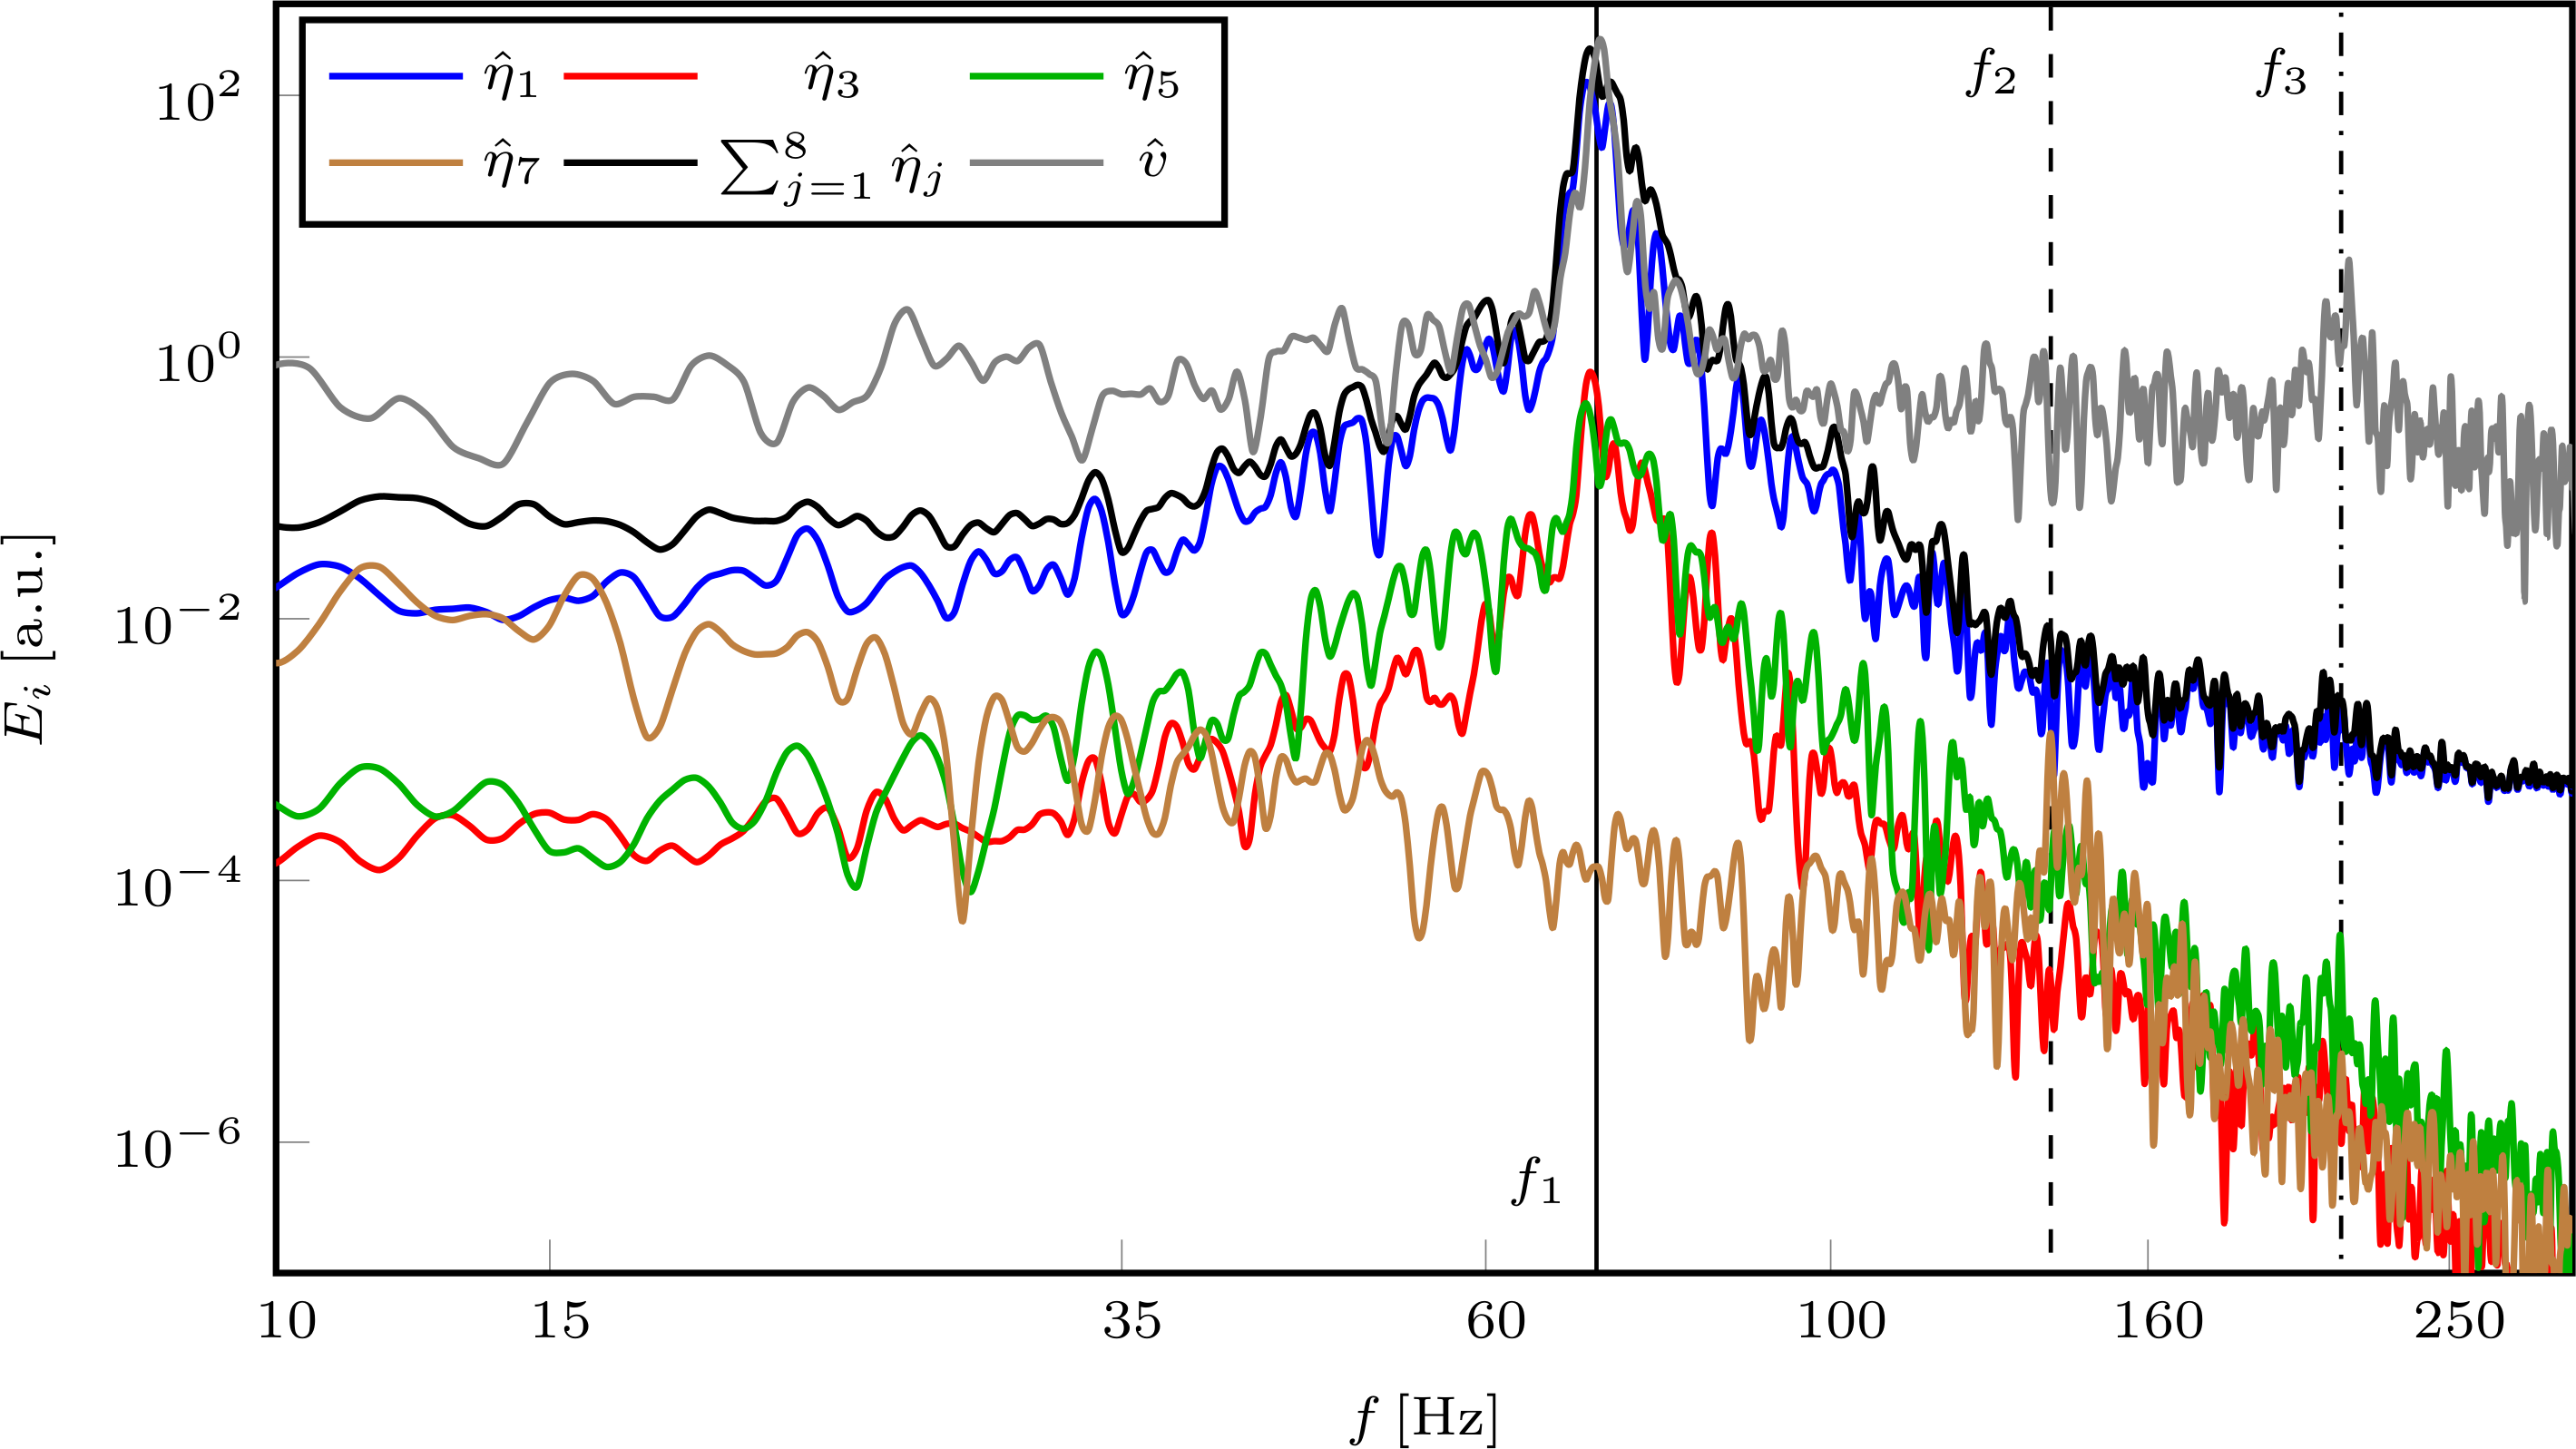
\includegraphics[width=0.98\textwidth]{02_images/00_export/figure27.png}
    \caption{Dynamics of vortex shedding behind a circular cylinder at $\Rey = 4815$. Spectra $\hat{\eta}_{j}$ obtained by the Fourier transform of $\eta_{i},\,i=1,3,5,6$, scaled by $\sigma_{i}^{2}$ and their sum, compared to the spectrum of $v$ velocity component in the point $p_{1}$ (see Figure~\ref{fig:meansPom1}). Spectra of $\eta_{j},\,j=2,4,6,8$, look qualitatively the same as spectra of their odd counterparts and were omitted for the sake of image clarity.}
    \label{fig:turbVKStreetSpectra}
\end{figure}
To further comment on the relation between the overal system and the POD modes dynamics, let us concentrate on the link between the chronoses spectra and their trajectories and integral curves. First, in Figure~\ref{fig:turbVKStreetSpectra}, we show a counterpart of Figure~\ref{fig:lamVKStreetSpectra}, but for the actually studied $\Rey = 4815$ and the fully three-dimensional data obtained via rPOD. Note the pronounced strong peaks in $\hat{v}_{p_{1}}$ spectra on the flow first and third harmonics and the absence of any peak at the second harmonics ($f_{2}$). However, the peak at $f_{2}$ may be identified in $\hat{u}_{p_{1}}$ and both $\hat{u}_{p_{2}}$ and $\hat{v}_{p_{2}}$, see Figure~\ref{fig:turbSpectraPts}. Furthermore, in the POD analysis of the turbulent flow, the first six modes oscillate primarily on the flow first harmonics. Still, the second flow harmonics is reconstructed by the seventh and eight 3D POD modes in a manner similar to the reconstruction of the second flow harmonics by the third and fourth modes in the 2D laminar von Karman vortex street.

\begin{figure}[tbp]
    \centering
    % \begin{tikzpicture}
	\begin{axis}[
		name=lamCase,
		xlabel={$\eta_{j}/\max{|\eta_{1}|}$},
		ylabel={$\eta_{j+1}/\max{|\eta_{1}|}$},
		font = \scriptsize,
		width=0.52\textwidth,
		height=0.52\textwidth,
		ytick pos=left,
		xtick pos=bottom,
		line width = 0.85pt,
        xmin=-1.05,
        xmax=1.05,
        ymin=-1.05,
        ymax=1.05,
        legend style ={
                at={(0.01,0.99)}, 
                anchor=north west,
                draw=black, 
                fill=white,
                align=right,
                legend columns=2,
                font=\scriptsize
            },
		]
		\addplot [color=blue,mark=none,select coords between index={1}{400},smooth] table [x expr=\thisrow{eta0}/2.14766, y expr = \thisrow{eta1}/2.14766]{\myGraphs/lamVKStreet/etas0-7Re115.dat};
        \addlegendentry{$j=1$};
		\addplot [color=red,mark=none,select coords between index={1}{400},smooth] table [x expr=\thisrow{eta2}/2.14766, y expr = \thisrow{eta3}/2.14766]{\myGraphs/lamVKStreet/etas0-7Re115.dat};
        \addlegendentry{$j=2$};
		\addplot [color=green!70!black,mark=none,select coords between index={1}{400},smooth] table [x expr=\thisrow{eta4}/2.14766, y expr = \thisrow{eta5}/2.14766]{\myGraphs/lamVKStreet/etas0-7Re115.dat};
        \addlegendentry{$j=3$};
		\addplot [color=brown,mark=none,select coords between index={1}{400},smooth] table [x expr=\thisrow{eta6}/2.14766, y expr = \thisrow{eta7}/2.14766]{\myGraphs/lamVKStreet/etas0-7Re115.dat};
        \addlegendentry{$j=4$};
	\end{axis}
	\begin{axis}[
		name=turbCase,
        at=(lamCase.east),
        anchor=west,
        xshift=0.1\textwidth,
		xlabel={$\eta_{j}/\max{|\eta_{1}|}$},
		font = \scriptsize,
		width=0.52\textwidth,
		height=0.52\textwidth,
		ytick pos=left,
		xtick pos=bottom,
		line width = 0.85pt,
        xmin=-1.05,
        xmax=1.05,
        ymin=-1.05,
        ymax=1.05,
		]
		\addplot [color=blue,mark=none,select coords between index={1}{400},smooth] table [x expr=\thisrow{eta0}/1861.34, y expr = \thisrow{eta1}/1861.34]{\myGraphs/lamVKStreet/3DTurbEtasV1.dat};
		\addplot [color=red,mark=none,select coords between index={1}{400},smooth] table [x expr=\thisrow{eta2}/1861.34, y expr = \thisrow{eta3}/1861.34]{\myGraphs/lamVKStreet/3DTurbEtasV1.dat};
		\addplot [color=green!70!black,mark=none,select coords between index={1}{400},smooth] table [x expr=\thisrow{eta4}/1861.34, y expr = \thisrow{eta5}/1861.34]{\myGraphs/lamVKStreet/3DTurbEtasV1.dat};
		\addplot [color=brown,mark=none,select coords between index={1}{400},smooth] table [x expr=\thisrow{eta6}/1861.34, y expr = \thisrow{eta7}/1861.34]{\myGraphs/lamVKStreet/3DTurbEtasV1.dat};
	\end{axis}
\end{tikzpicture}

    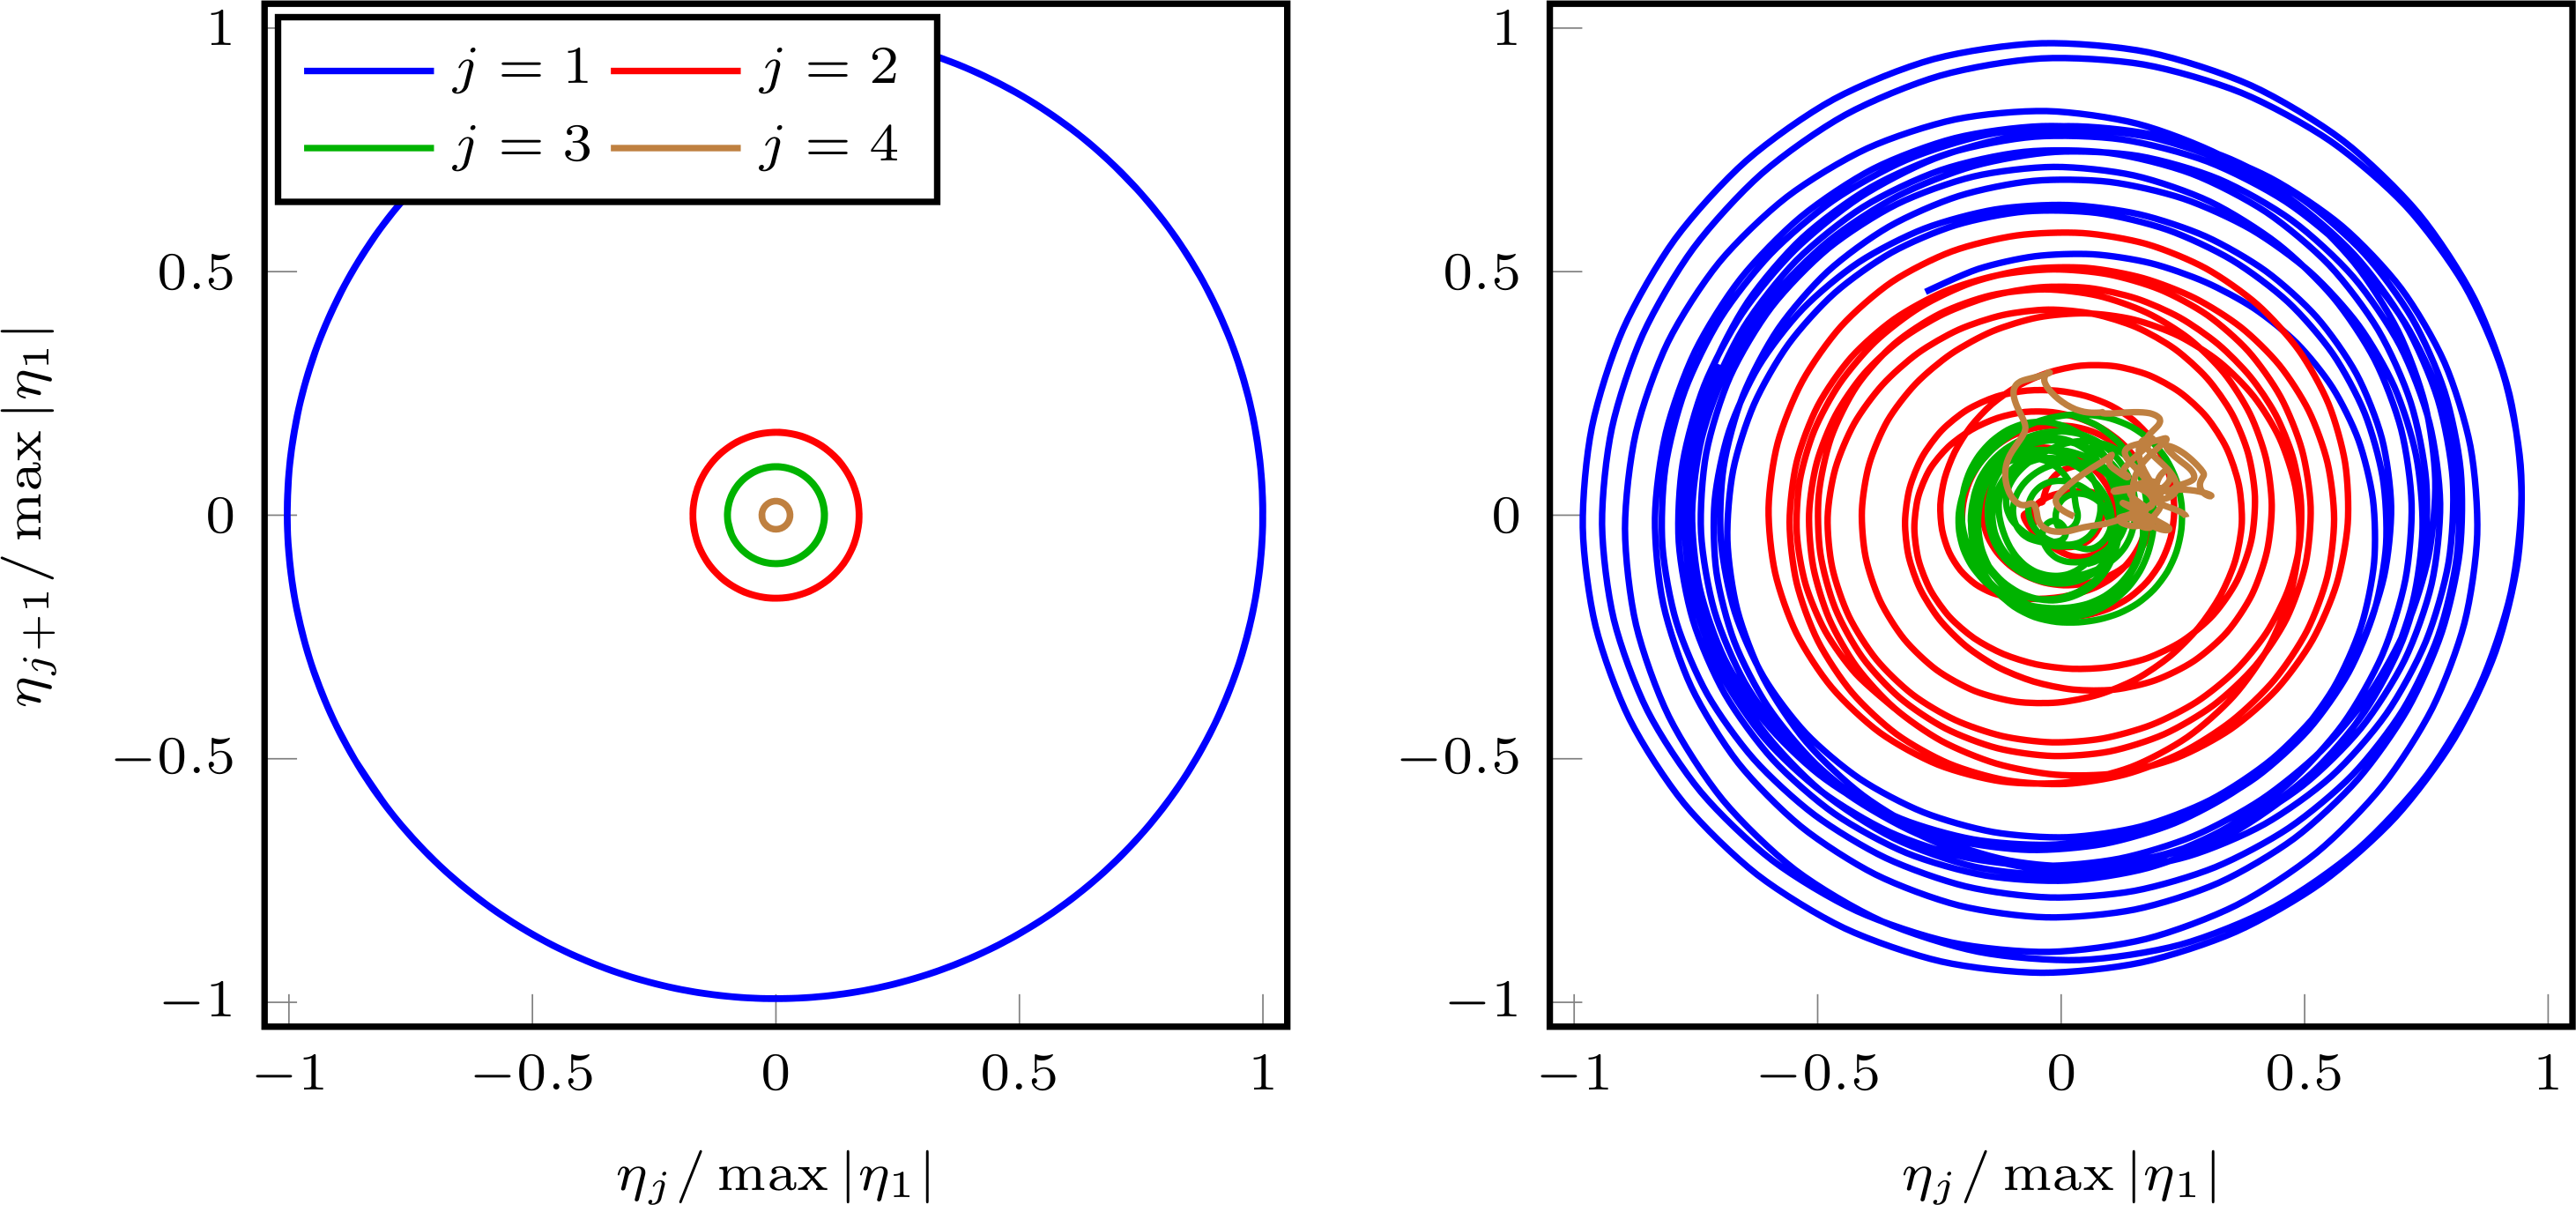
\includegraphics[width=0.98\textwidth]{02_images/00_export/figure28.png}
    \caption{Trajectories of the first four mode pairs chronoses for the laminar (left) and turbulent (right) case of vortex shedding behind a circular cylinder in a cross flow at $\Rey = 115$ and $\Rey = 4815$, respectively. The chronos amplitudes are scaled by the amplitude of the first mode chronos.}
    \label{fig:appEtasLam}
\end{figure}
Also, note the more pronounced and random oscillations in the spectra of turbulent flow chronoses accompanied by a less steep energy decay  compared to the laminar case. The actual trajectories of the chronoses of the first four mode pairs for both the laminar and the turbulent cases are given in Figure~\ref{fig:appEtasLam}. The trajectories of the laminar POD chronoses are periodic with periods corresponding to the flow harmonics, and form circles in the $\eta_{j}-\eta_{j+1}, j = 1,3,5,7$ planes. Such a behavior is in agreement with the theoretical analysis of the von Karman vortex street formation based on the theory of dynamical systems, in which the transition from a steady-state flow at extremely low $\Rey$ to a vortex street is identified with a Hopf bifurcation leading to a stable periodic system trajectory \cite{williamson1996}.

The trajectories of the first four chronos pairs obtained from POD analysis of the turbulent flow are shown in the right hand side of Figure~\ref{fig:appEtasLam}. Especially the first three pairs behave in a manner similar to the laminar case. Albeit, the trajectories of chronos pairs are now only quasi-periodic and their amplitudes oscillate. Such a behavior is in agreement with the quasi-laminar behavior of the low POD modes. The trajectory of the fourth chronos pair is seemingly random. However, based on the spectra similarity between the turbulent and the laminar cases, it would be reasonable to expect the fourth mode pair to exhibit at least somehow regular dynamics.


\begin{figure}[tbp]
    \centering
    % \begin{tikzpicture}
	\begin{axis}[
		name=lamCase,
		%~ xlabel={$t$},
		ylabel={$\eta_{j}/\max{|\eta_{j}|}$},
		font = \scriptsize,
		width=0.98\textwidth,
		height=0.52\textwidth,
		ytick pos=left,
		xtick pos=bottom,
		line width = 0.85pt,
        xmin=0,
        xmax=6,
        ymin=-1.05,
        ymax=1.05,
		]
		\addplot [color=blue,mark=none,select coords between index={1}{300},smooth] table [x expr=\thisrow{t}/0.666666, y expr = \thisrow{eta0}/2.14766]{\myGraphs/lamVKStreet/etas0-7Re115.dat};
		\addplot [color=red,mark=none,select coords between index={1}{300},smooth] table [x expr=\thisrow{t}/0.666666, y expr = \thisrow{eta2}/0.36769]{\myGraphs/lamVKStreet/etas0-7Re115.dat};
		\addplot [color=green!70!black,mark=none,select coords between index={1}{300},smooth] table [x expr=\thisrow{t}/0.666666, y expr = \thisrow{eta4}/0.2153]{\myGraphs/lamVKStreet/etas0-7Re115.dat};
		\addplot [color=brown,mark=none,select coords between index={1}{300},smooth] table [x expr=\thisrow{t}/0.666666, y expr = \thisrow{eta6}/0.0627083]{\myGraphs/lamVKStreet/etas0-7Re115.dat};
	\end{axis}
    \begin{axis}[
		name=turbCase,
        anchor=north,
        at=(lamCase.below south),
		xlabel={$\tilde{t}$},
		ylabel={$\eta_{j}/\max{|\eta_{j}|}$},
		font = \scriptsize,
		width=0.98\textwidth,
		height=0.52\textwidth,
		ytick pos=left,
		xtick pos=bottom,
		line width = 0.85pt,
        xmin=0,
        xmax=6,
        ymin=-1.05,
        ymax=1.05,
        legend style ={
                at={(0.01,0.99)}, 
                anchor=north west,
                draw=black, 
                fill=white,
                align=right,
                legend columns=4,
                font=\scriptsize
            },
		]
		\addplot [color=blue,mark=none,select coords between index={1}{200}] table [x expr=\thisrow{t}/0.014064697609001408, y expr = \thisrow{eta0}/1861.34]{\myGraphs/lamVKStreet/3DTurbEtasV1.dat};
        \addlegendentry{$j=1$};
		\addplot [color=red,mark=none,select coords between index={1}{200}] table [x expr=\thisrow{t}/0.014064697609001408, y expr = \thisrow{eta2}/1540.7]{\myGraphs/lamVKStreet/3DTurbEtasV1.dat};
        \addlegendentry{$j=3$};
		\addplot [color=green!70!black,mark=none,select coords between index={1}{200}] table [x expr=\thisrow{t}/0.014064697609001408, y expr = \thisrow{eta4}/877.636]{\myGraphs/lamVKStreet/3DTurbEtasV1.dat};
        \addlegendentry{$j=5$};
		\addplot [color=brown,mark=none,select coords between index={1}{200}] table [x expr=\thisrow{t}/0.014064697609001408, y expr = \thisrow{eta6}/638.358]{\myGraphs/lamVKStreet/3DTurbEtasV1.dat};
        \addlegendentry{$j=7$};
	\end{axis}
\end{tikzpicture}

    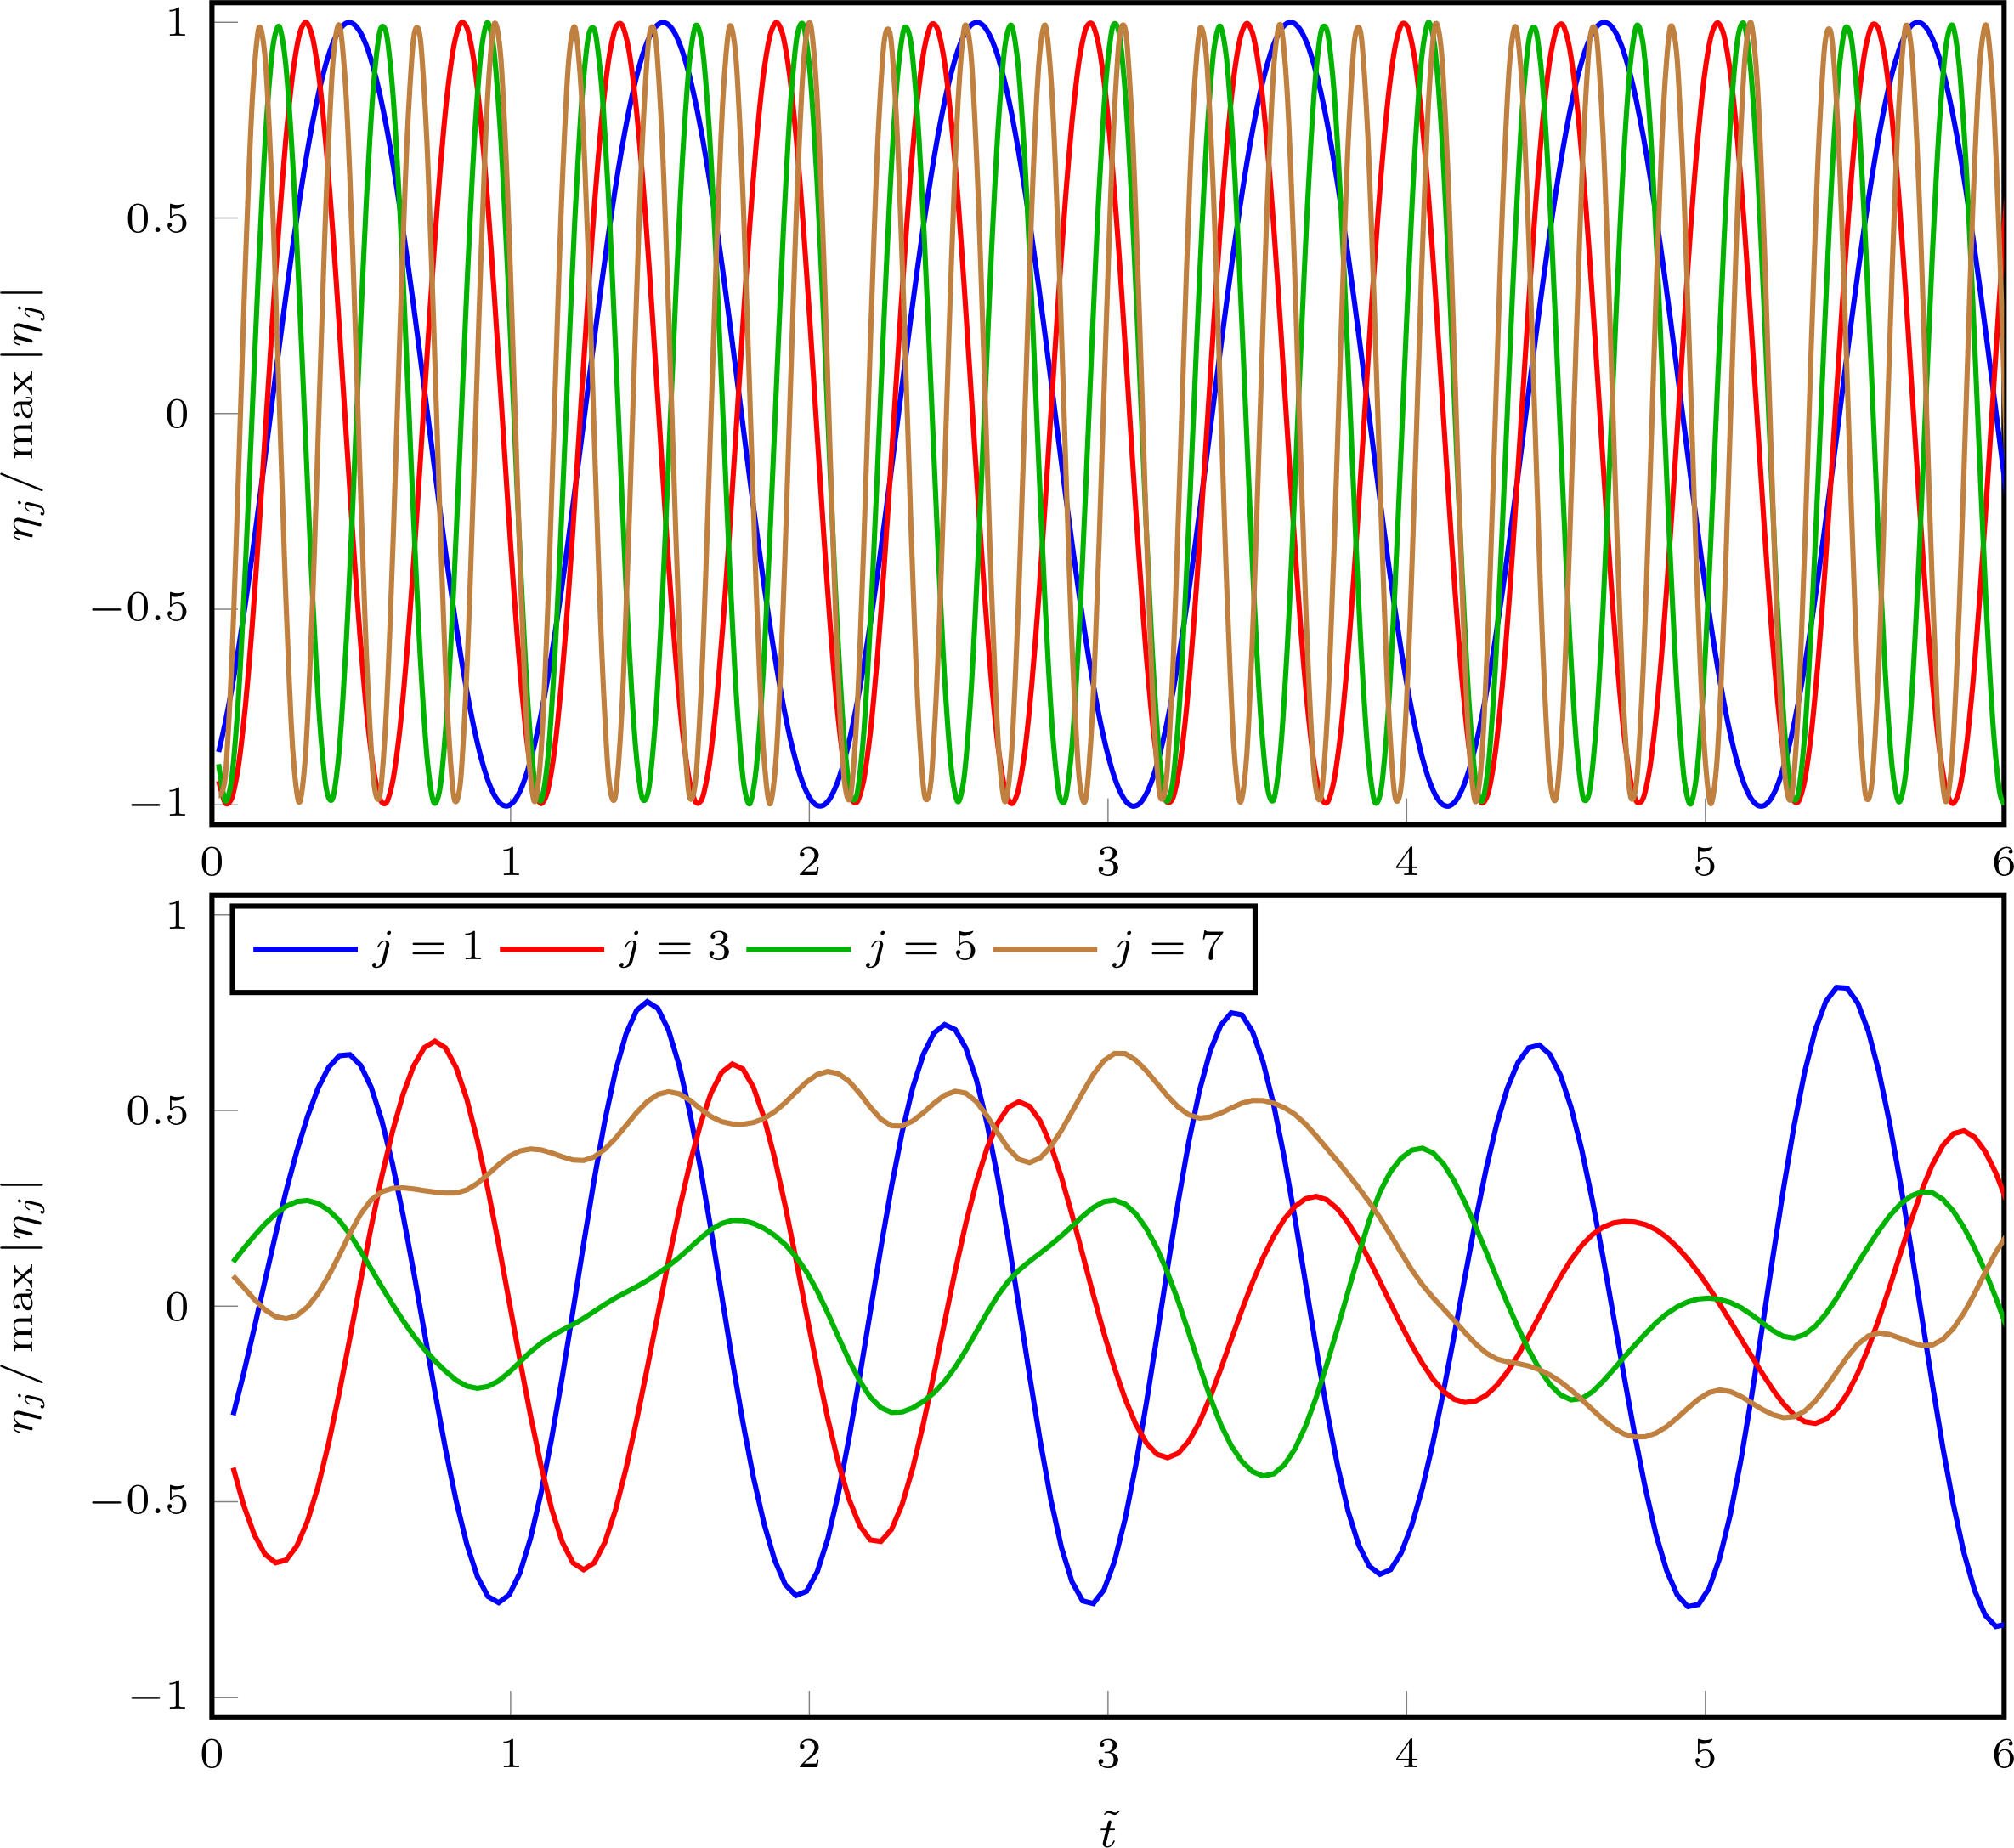
\includegraphics[width=0.98\textwidth]{02_images/00_export/figure29.png}
    \caption{Integral curves of the first, third, fifth and seventh mode chronoses over six principal flow periods, $\tilde{t} = t/T_{1}$, $T_{1} = 1/f_{1}$ for the laminar (top) and turbulent (bottom) case. The chronoses are scaled by their amplitudes.}
    \label{fig:appEtasLamInt}
\end{figure}
The regularity of the fourth mode pair dynamics is hinted at in Figure~\ref{fig:appEtasLamInt}, where the integral curves of selected chronoses are depicted. As a reference, scaled integral curves of the chronoses 1, 3, 5, and 7, which correspond to a periodic flow behavior, are shown in the top part of the figure. The integral curve of $\eta_{1}$ obtained from the performed POD analysis of the turbulent flow behaves qualitatively similar to its laminar counterpart, compare the blue curves in Figure~\ref{fig:appEtasLamInt}. In particular, it oscillates rather regularly with a scaled amplitude ranging from 0.65 to 1.0. Next, $\eta_{3}$ and $\eta_{5}$ extracted from the turbulent flow complement $\eta_{1}$ in creation of the oblique, and as such three-dimensional, laminar-like vortex shedding, see section~\ref{sub:partRec}. Consequently, it may be seen that they oscillate primarily at the same frequency as $\eta_{1}$. Still, the variance in their scaled apmlitudes is more pronounced. Finally, $\eta_{7}$ based on the turbulent flow analysis exhibits low-frequency but high-amplitude oscillations combined with low amplitude oscillations at the frequency $f_{2}$. While the frequency of high-amplitude oscillation changes, the low-amplitude oscillations are regular, which results in the spectrum shown in Figure~\ref{fig:turbVKStreetSpectra}.

% section fourier (end)
